\documentclass[aspectratio=169]{beamer}

% -------------------------
% Basic packages
% -------------------------
\usepackage[utf8]{inputenc}
\usepackage{graphicx}
\usepackage{amsmath, amssymb}
\usepackage{booktabs}
\usepackage{array}
\usepackage{tikz}
\usepackage{tcolorbox}
\usepackage{hyperref}
\definecolor{questionbg}{RGB}{235, 244, 255}
\definecolor{questionframe}{RGB}{44, 95, 173}
\definecolor{plainbg}{RGB}{241, 249, 241}
\definecolor{plainframe}{RGB}{44, 122, 70}
\definecolor{notationbg}{RGB}{255, 248, 230}
\definecolor{notationframe}{RGB}{176, 118, 0}

\newtcolorbox{questionbox}{
  colback=questionbg,
  colframe=questionframe,
  boxrule=0.7pt,
  arc=1mm,
  fontupper=\small,
  left=1mm,
  right=1mm,
  top=0.4mm,
  bottom=0.4mm
}

\newtcolorbox{plainbox}{
  colback=plainbg,
  colframe=plainframe,
  boxrule=0.7pt,
  arc=1mm,
  fontupper=\small,
  left=1mm,
  right=1mm,
  top=0.4mm,
  bottom=0.4mm
}

\newtcolorbox{notationbox}{
  colback=notationbg,
  colframe=notationframe,
  boxrule=0.7pt,
  arc=1mm,
  fontupper=\small,
  left=1mm,
  right=1mm,
  top=0.4mm,
  bottom=0.4mm
}

\newcommand{\keyquestion}[1]{%
  \begin{questionbox}
  \textbf{Question:} #1
  \end{questionbox}
}

\newcommand{\plainidea}[1]{%
  \begin{plainbox}
  \textbf{Main idea:} #1
  \end{plainbox}
}

\newcommand{\notationblock}[1]{%
  \begin{notationbox}
  \textbf{Symbols used on this slide}\\
  #1
  \end{notationbox}
}

\newcommand{\exercisebreakcontent}[1]{%
  \begin{center}
  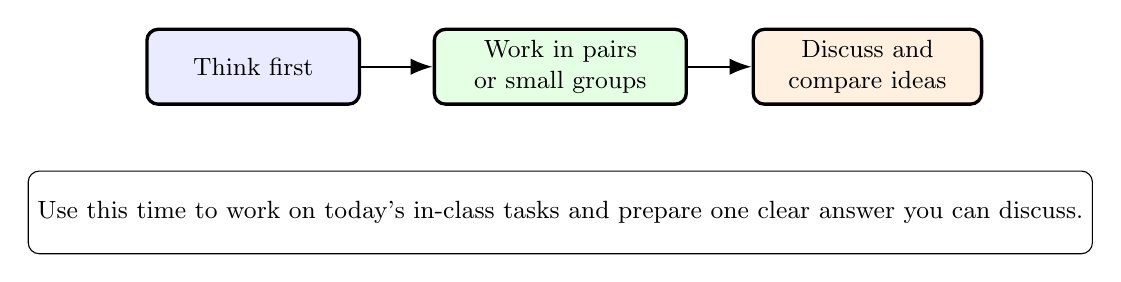
\begin{tikzpicture}[>=Latex, every node/.style={font=\small}]
    \node[draw, rounded corners, very thick, fill=blue!8, minimum width=2.7cm, minimum height=0.95cm, align=center] (think) at (-3.9,0.9) {Think first};
    \node[draw, rounded corners, very thick, fill=green!10, minimum width=3.2cm, minimum height=0.95cm, align=center] (work) at (0,0.9) {Work in pairs\\or small groups};
    \node[draw, rounded corners, very thick, fill=orange!12, minimum width=2.9cm, minimum height=0.95cm, align=center] (share) at (3.9,0.9) {Discuss and\\compare ideas};
    \draw[-{Latex[length=2.8mm]}, thick] (think) -- (work);
    \draw[-{Latex[length=2.8mm]}, thick] (work) -- (share);
    \node[draw, rounded corners, fill=white, minimum width=9.4cm, minimum height=1.05cm, align=center] at (0,-0.95) {Use this time to work on today's in-class tasks and prepare one clear answer you can discuss.};
  \end{tikzpicture}
  \end{center}
  \plainidea{#1}
}

\usetikzlibrary{positioning,arrows.meta,fit,calc}

% -------------------------
% Theme
% -------------------------
\usetheme{Madrid}
\usecolortheme{default}
\setbeamertemplate{navigation symbols}{}

% -------------------------
% Per-slide reference footer
% -------------------------
\newcommand{\defaultdeckrefs}{AIMA4e Ch.14 pp.461--499; Poole3e Ch.9 pp.375--458}
\newcommand{\currentsliderefs}{\defaultdeckrefs}
\newcommand{\setslideref}[1]{\gdef\currentsliderefs{#1}}
\addtobeamertemplate{footline}{}{%
  \begin{beamercolorbox}[wd=\paperwidth,leftskip=0.4em,rightskip=0.4em,ht=2.8ex,dp=0.9ex]{author in head/foot}
    \tiny\textbf{Refs: }\currentsliderefs
  \end{beamercolorbox}
}

% -------------------------
% Metadata
% -------------------------
\title[EBU6505 B4 D3]{EBU6505 -- Reasoning and Agents\\Block 4, Day 3 -- Probabilistic Reasoning over Time}
\author{Dr Riasat Islam}
\institute{Queen Mary University of London}
\date{}

% -------------------------
% TikZ styles
% -------------------------
\tikzset{
  flowarrow/.style={-{Latex[length=2.8mm]}, thick},
  softarrow/.style={-{Latex[length=2.4mm]}, thick, gray!70},
  statenode/.style={draw, rounded corners, very thick, fill=blue!10, minimum width=2.15cm, minimum height=0.95cm, align=center},
  evidnode/.style={draw, rounded corners, very thick, fill=green!12, minimum width=2.15cm, minimum height=0.95cm, align=center},
  hiddennode/.style={draw, rounded corners, very thick, fill=orange!12, minimum width=2.15cm, minimum height=0.95cm, align=center},
  softbox/.style={draw, rounded corners, fill=white, minimum width=2.7cm, minimum height=0.95cm, align=center},
  note/.style={draw, rounded corners, fill=white, minimum width=3.0cm, minimum height=0.95cm, align=center},
  relabel/.style={font=\small, fill=white, inner sep=1pt}
}

\begin{document}

\setslideref{AIMA4e Ch.14 pp.461--499; Poole3e Ch.9 pp.375--458}
\begin{frame}
  \titlepage
\end{frame}

\begin{frame}{What have we covered this week?}
\begin{itemize}
  \item Day 1: Bayesian networks for uncertain reasoning
  \item Day 2: exact inference with enumeration and variable elimination
  \item elimination order and treewidth as cost intuition
\end{itemize}
\plainidea{So far the model has been static. Today we ask what happens when the hidden state changes over time.}
\end{frame}

\begin{frame}{What are we going to cover this week?}
\begin{itemize}
  \item Day 1: Bayesian networks
  \item Day 2: exact inference in Bayesian networks
  \item Day 3: probabilistic reasoning over time
  \item Day 4: planning with uncertainty
  \item Day 5: dynamic decision networks and partially observable Markov decision process synthesis
\end{itemize}
\plainidea{This week moves from static uncertain belief to temporal belief, and then from belief to action.}
\end{frame}

\begin{frame}{What are we going to cover today?}
\begin{itemize}
  \item why time makes probabilistic reasoning harder
  \item one simple running example: rain and umbrella
  \item filtering, prediction, smoothing, and most likely sequence
  \item hidden Markov models (HMMs), Kalman filters, and dynamic Bayesian networks (DBNs)
  \item exact versus approximate inference in temporal models
\end{itemize}
\plainidea{The whole lecture answers one question: how do we track a hidden state when the world keeps changing?}
\end{frame}

\begin{frame}{Resources}
\small
\begin{itemize}
  \item \textit{Artificial Intelligence: A Modern Approach}, Russell and Norvig (4th ed.)
  \item AIMA 4e, Chapter 14: Probabilistic Reasoning over Time
  \item \textit{Artificial Intelligence: Foundations of Computational Agents}, David Poole and Alan Mackworth (3rd ed.)
  \item Poole 3e, Chapter 9: Reasoning with Uncertainty
  \item Focus section for Poole: sequential probability models
\end{itemize}
\plainidea{Both textbooks use the same core idea: the hidden state changes over time, but we only observe noisy evidence about it.}
\end{frame}

\begin{frame}{Learning Outcomes for Today}
\begin{itemize}
  \item explain why temporal reasoning is different from one-shot inference
  \item explain filtering, prediction, smoothing, and most likely sequence
  \item read the structure of a hidden Markov model (HMM) and a dynamic Bayesian network (DBN)
  \item explain when Kalman filters are more suitable than discrete hidden Markov models
  \item explain why approximate inference is often needed in larger temporal models
\end{itemize}
\plainidea{If these five ideas are clear, students can follow the temporal-model lectures without getting buried in notation.}
\end{frame}

\begin{frame}{Warm-Up Question}
\keyquestion{If you see umbrellas on three days in a row, what can you say about the rain on the third day?}
\begin{columns}[T,onlytextwidth]
  \begin{column}{0.50\textwidth}
    \begin{center}
    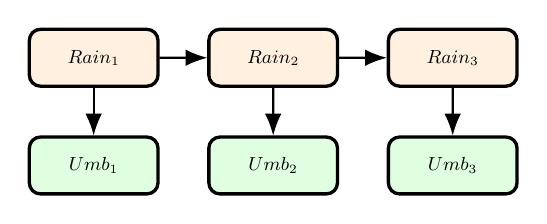
\begin{tikzpicture}[>=Latex, scale=0.76, every node/.style={font=\small, transform shape}]
      \node[hiddennode] (r1) at (0,1.1) {$Rain_1$};
      \node[evidnode] (u1) at (0,-0.7) {$Umb_1$};
      \node[hiddennode] (r2) at (3.0,1.1) {$Rain_2$};
      \node[evidnode] (u2) at (3.0,-0.7) {$Umb_2$};
      \node[hiddennode] (r3) at (6.0,1.1) {$Rain_3$};
      \node[evidnode] (u3) at (6.0,-0.7) {$Umb_3$};
      \draw[flowarrow] (r1) -- (r2);
      \draw[flowarrow] (r2) -- (r3);
      \draw[flowarrow] (r1) -- (u1);
      \draw[flowarrow] (r2) -- (u2);
      \draw[flowarrow] (r3) -- (u3);
    \end{tikzpicture}
    \end{center}
  \end{column}
  \begin{column}{0.46\textwidth}
    \begin{tcolorbox}[colback=questionbg,colframe=questionframe,boxrule=0.7pt,title=What is hidden?]
    Whether it is raining each day.
    \end{tcolorbox}
    \begin{tcolorbox}[colback=plainbg,colframe=plainframe,boxrule=0.7pt,title=What is observed?]
    Whether someone carries an umbrella each day.
    \end{tcolorbox}
  \end{column}
\end{columns}
\plainidea{One observation can influence belief across several time steps.}
\end{frame}

\begin{frame}{Why Is Time a New Challenge?}
\keyquestion{Why is one static Bayesian network not enough for a changing world?}
\begin{columns}[T,onlytextwidth]
  \begin{column}{0.48\textwidth}
    \begin{tcolorbox}[colback=questionbg,colframe=questionframe,boxrule=0.7pt,title=Static case]
    one snapshot\\
    one set of variables\\
    one inference question
    \end{tcolorbox}
  \end{column}
  \begin{column}{0.48\textwidth}
    \begin{tcolorbox}[colback=plainbg,colframe=plainframe,boxrule=0.7pt,title=Temporal case]
    hidden state changes\\
    new evidence keeps arriving\\
    belief must be updated again
    \end{tcolorbox}
  \end{column}
\end{columns}
\begin{center}
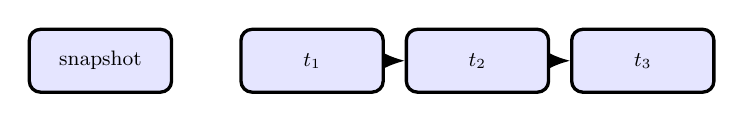
\begin{tikzpicture}[>=Latex, scale=0.84, every node/.style={font=\small, transform shape}]
  \node[statenode] (s) at (0,0) {snapshot};
  \node[statenode] (t1) at (3.2,0) {$t_1$};
  \node[statenode] (t2) at (5.7,0) {$t_2$};
  \node[statenode] (t3) at (8.2,0) {$t_3$};
  \draw[flowarrow] (t1) -- (t2);
  \draw[flowarrow] (t2) -- (t3);
\end{tikzpicture}
\end{center}
\plainidea{With time, inference becomes a repeated belief-update process.}
\end{frame}

\begin{frame}{Our Running Example: Rain and Umbrella}
\keyquestion{What are the state and evidence variables in the simplest temporal model?}
\begin{columns}[T,onlytextwidth]
  \begin{column}{0.50\textwidth}
    \begin{tcolorbox}[colback=plainbg,colframe=plainframe,boxrule=0.7pt,title=Hidden state]
    $Rain_t$\\
    rain or no rain at time $t$
    \end{tcolorbox}
    \begin{tcolorbox}[colback=questionbg,colframe=questionframe,boxrule=0.7pt,title=Evidence]
    $Umb_t$\\
    umbrella or no umbrella at time $t$
    \end{tcolorbox}
  \end{column}
  \begin{column}{0.46\textwidth}
    \begin{center}
    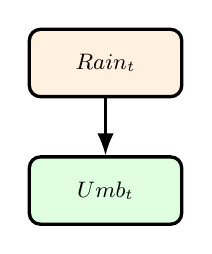
\begin{tikzpicture}[>=Latex, scale=0.9, every node/.style={font=\small, transform shape}]
      \node[hiddennode] (r) at (0,0.9) {$Rain_t$};
      \node[evidnode] (u) at (0,-0.9) {$Umb_t$};
      \draw[flowarrow] (r) -- (u);
    \end{tikzpicture}
    \end{center}
  \end{column}
\end{columns}
\plainidea{We do not see the weather directly. We only see evidence about it.}
\end{frame}

\begin{frame}{How Do We Connect One Day to the Next?}
\keyquestion{What dependencies appear when we move from one time step to many?}
\begin{center}
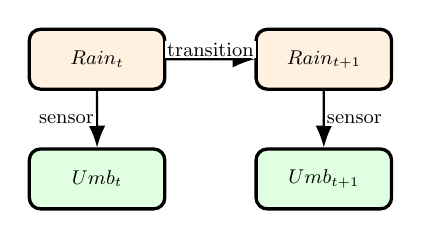
\begin{tikzpicture}[>=Latex, scale=0.80, every node/.style={font=\small, transform shape}]
  \node[hiddennode] (r1) at (0,1.1) {$Rain_t$};
  \node[evidnode] (u1) at (0,-0.8) {$Umb_t$};
  \node[hiddennode] (r2) at (3.6,1.1) {$Rain_{t+1}$};
  \node[evidnode] (u2) at (3.6,-0.8) {$Umb_{t+1}$};
  \draw[flowarrow] (r1) -- node[relabel, above] {transition} (r2);
  \draw[flowarrow] (r1) -- node[relabel, left] {sensor} (u1);
  \draw[flowarrow] (r2) -- node[relabel, right] {sensor} (u2);
\end{tikzpicture}
\end{center}
\vspace{-0.4em}
\begin{columns}[T,onlytextwidth]
  \begin{column}{0.48\textwidth}
    \begin{tcolorbox}[colback=plainbg,colframe=plainframe,boxrule=0.7pt,title=Transition model]
    How likely is tomorrow's state given today's state?
    \end{tcolorbox}
  \end{column}
  \begin{column}{0.48\textwidth}
    \begin{tcolorbox}[colback=questionbg,colframe=questionframe,boxrule=0.7pt,title=Sensor model]
    How likely is the observation, given the hidden state?
    \end{tcolorbox}
  \end{column}
\end{columns}
\plainidea{A temporal model needs a state-change model and an observation model.}
\end{frame}

\begin{frame}{Four Core Temporal Questions}
\keyquestion{What kinds of inference questions do we ask over time?}
\small
\begin{columns}[T,onlytextwidth]
  \begin{column}{0.48\textwidth}
    \begin{tcolorbox}[colback=plainbg,colframe=plainframe,boxrule=0.7pt,title=Filtering]
    What do we believe about the hidden state now?
    \end{tcolorbox}
    \begin{tcolorbox}[colback=questionbg,colframe=questionframe,boxrule=0.7pt,title=Prediction]
    What do we believe about the hidden state later?
    \end{tcolorbox}
  \end{column}
  \begin{column}{0.48\textwidth}
    \begin{tcolorbox}[colback=notationbg,colframe=notationframe,boxrule=0.7pt,title=Smoothing]
    What do we believe about an earlier state after later evidence?
    \end{tcolorbox}
    \begin{tcolorbox}[colback=plainbg,colframe=plainframe,boxrule=0.7pt,title=Most likely sequence]
    What is the single best full hidden-state path?
    \end{tcolorbox}
  \end{column}
\end{columns}
\plainidea{These four questions organise the whole lecture.}
\end{frame}

\begin{frame}{Filtering}
\keyquestion{What do we believe about the hidden state right now?}
\begin{columns}[T,onlytextwidth]
  \begin{column}{0.54\textwidth}
    \[
    P(Rain_t \mid umb_1,\ldots,umb_t)
    \]
    \begin{tcolorbox}[colback=plainbg,colframe=plainframe,boxrule=0.7pt,title=Simple meaning]
    Use all evidence up to today to estimate today's hidden state.
    \end{tcolorbox}
    \begin{tcolorbox}[colback=questionbg,colframe=questionframe,boxrule=0.7pt,title=Example question,fontupper=\small]
    After three umbrella days, how likely is rain today?
    \end{tcolorbox}
  \end{column}
  \begin{column}{0.42\textwidth}
    \begin{center}
    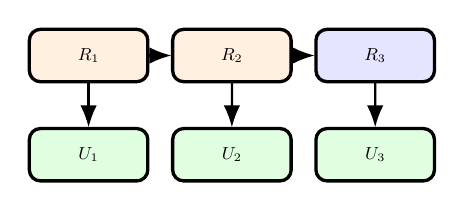
\begin{tikzpicture}[>=Latex, scale=0.70, every node/.style={font=\small, transform shape}]
      \node[hiddennode] (r1) at (0,1.1) {$R_1$};
      \node[evidnode] (u1) at (0,-0.7) {$U_1$};
      \node[hiddennode] (r2) at (2.6,1.1) {$R_2$};
      \node[evidnode] (u2) at (2.6,-0.7) {$U_2$};
      \node[statenode] (r3) at (5.2,1.1) {$R_3$};
      \node[evidnode] (u3) at (5.2,-0.7) {$U_3$};
      \draw[flowarrow] (r1) -- (r2);
      \draw[flowarrow] (r2) -- (r3);
      \draw[flowarrow] (r1) -- (u1);
      \draw[flowarrow] (r2) -- (u2);
      \draw[flowarrow] (r3) -- (u3);
    \end{tikzpicture}
    \end{center}
  \end{column}
\end{columns}
\vspace{-0.3em}
\plainidea{Filtering asks about the current hidden state.}
\end{frame}

\begin{frame}{Filtering Uses Two Steps}
\keyquestion{How do we update today's belief from yesterday's belief?}
\begin{center}
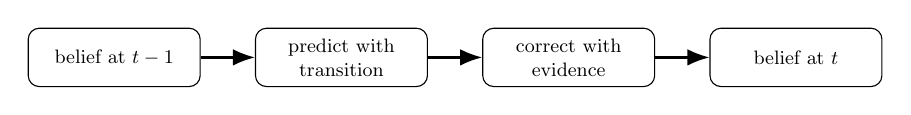
\begin{tikzpicture}[>=Latex, scale=0.78, every node/.style={font=\small, transform shape}]
  \node[softbox, minimum width=2.8cm] (old) at (0,0) {belief at $t-1$};
  \node[softbox, minimum width=2.8cm] (pred) at (3.7,0) {predict with\\transition};
  \node[softbox, minimum width=2.8cm] (corr) at (7.4,0) {correct with\\evidence};
  \node[softbox, minimum width=2.8cm] (new) at (11.1,0) {belief at $t$};
  \draw[flowarrow] (old) -- (pred);
  \draw[flowarrow] (pred) -- (corr);
  \draw[flowarrow] (corr) -- (new);
\end{tikzpicture}
\end{center}
\begin{columns}[T,onlytextwidth]
  \begin{column}{0.48\textwidth}
    \begin{tcolorbox}[colback=plainbg,colframe=plainframe,boxrule=0.7pt,title=Predict step]
    Move the belief forward with the transition model.
    \end{tcolorbox}
  \end{column}
  \begin{column}{0.48\textwidth}
    \begin{tcolorbox}[colback=questionbg,colframe=questionframe,boxrule=0.7pt,title=Correct step]
    Adjust the belief using the observation seen today.
    \end{tcolorbox}
  \end{column}
\end{columns}
\plainidea{Filtering repeats the same loop: predict first, then correct.}
\end{frame}

\begin{frame}{Prediction}
\keyquestion{What do we believe about a future hidden state if no new evidence arrives?}
\begin{columns}[T,onlytextwidth]
  \begin{column}{0.54\textwidth}
    \[
    P(Rain_{t+k} \mid umb_1,\ldots,umb_t)
    \]
    \begin{tcolorbox}[colback=plainbg,colframe=plainframe,boxrule=0.7pt,title=Simple meaning]
    Start from the current belief and move it forward with the transition model.
    \end{tcolorbox}
  \end{column}
  \begin{column}{0.42\textwidth}
    \begin{center}
    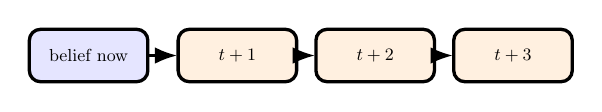
\begin{tikzpicture}[>=Latex, scale=0.70, every node/.style={font=\small, transform shape}]
      \node[statenode] (now) at (0,0) {belief now};
      \node[hiddennode] (n1) at (2.7,0) {$t+1$};
      \node[hiddennode] (n2) at (5.2,0) {$t+2$};
      \node[hiddennode] (n3) at (7.7,0) {$t+3$};
      \draw[flowarrow] (now) -- (n1);
      \draw[flowarrow] (n1) -- (n2);
      \draw[flowarrow] (n2) -- (n3);
    \end{tikzpicture}
    \end{center}
  \end{column}
\end{columns}
\plainidea{Prediction is a future-question.}
\end{frame}

\begin{frame}{Smoothing}
\keyquestion{How can later evidence help us revise our belief about an earlier hidden state?}
\begin{columns}[T,onlytextwidth]
  \begin{column}{0.54\textwidth}
    \[
    P(Rain_k \mid umb_1,\ldots,umb_T),\quad k<T
    \]
    \begin{tcolorbox}[colback=questionbg,colframe=questionframe,boxrule=0.7pt,title=Simple meaning]
    Use evidence from before and after time $k$ to improve the estimate for time $k$.
    \end{tcolorbox}
  \end{column}
  \begin{column}{0.42\textwidth}
    \begin{center}
    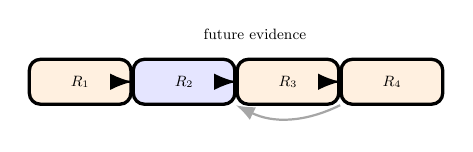
\begin{tikzpicture}[>=Latex, scale=0.60, every node/.style={font=\small, transform shape}]
      \node[hiddennode] (r1) at (0,0.8) {$R_1$};
      \node[statenode] (r2) at (2.2,0.8) {$R_2$};
      \node[hiddennode] (r3) at (4.4,0.8) {$R_3$};
      \node[hiddennode] (r4) at (6.6,0.8) {$R_4$};
      \draw[flowarrow] (r1) -- (r2);
      \draw[flowarrow] (r2) -- (r3);
      \draw[flowarrow] (r3) -- (r4);
      \draw[softarrow] (r4.south west) to[bend left=26] (r2.south east);
      \node[relabel] at (3.7,1.8) {future evidence};
    \end{tikzpicture}
    \end{center}
  \end{column}
\end{columns}
\plainidea{Smoothing improves a past estimate using later evidence.}
\end{frame}

\begin{frame}{Most Likely Sequence}
\keyquestion{What is the single best full hidden-state path across the whole timeline?}
\begin{columns}[T,onlytextwidth]
  \begin{column}{0.54\textwidth}
    \begin{tcolorbox}[colback=plainbg,colframe=plainframe,boxrule=0.7pt,title=Different from smoothing]
    Smoothing estimates each time step separately.\\[0.25em]
    Viterbi picks one best full sequence.
    \end{tcolorbox}
    \begin{tcolorbox}[colback=questionbg,colframe=questionframe,boxrule=0.7pt,title=Example]
    Example path: rain $\rightarrow$ rain $\rightarrow$ dry $\rightarrow$ dry
    \end{tcolorbox}
  \end{column}
  \begin{column}{0.42\textwidth}
    \begin{center}
    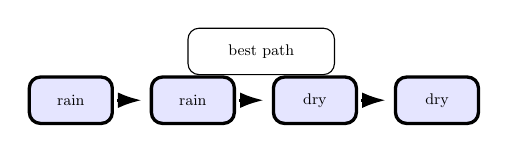
\begin{tikzpicture}[>=Latex, scale=0.62, every node/.style={font=\small, transform shape}]
      \node[note] at (3.9,1.0) {best path};
      \node[statenode, minimum width=1.7cm] (s1) at (0,0) {rain};
      \node[statenode, minimum width=1.7cm] (s2) at (2.5,0) {rain};
      \node[statenode, minimum width=1.7cm] (s3) at (5.0,0) {dry};
      \node[statenode, minimum width=1.7cm] (s4) at (7.5,0) {dry};
      \draw[-{Latex[length=3mm,width=2mm]}, line width=1pt] ($(s1.east)+(0.08,0)$) -- ($(s2.west)+(-0.18,0)$);
      \draw[-{Latex[length=3mm,width=2mm]}, line width=1pt] ($(s2.east)+(0.08,0)$) -- ($(s3.west)+(-0.18,0)$);
      \draw[-{Latex[length=3mm,width=2mm]}, line width=1pt] ($(s3.east)+(0.08,0)$) -- ($(s4.west)+(-0.18,0)$);
    \end{tikzpicture}
    \end{center}
  \end{column}
\end{columns}
\plainidea{Viterbi chooses one best complete hidden-state path.}
\end{frame}

\begin{frame}{How Do the Four Questions Differ?}
\keyquestion{How can we compare filtering, prediction, smoothing, and Viterbi quickly?}
\small
\begin{center}
\begin{tabular}{>{\raggedright\arraybackslash}p{0.20\textwidth} >{\raggedright\arraybackslash}p{0.30\textwidth} >{\raggedright\arraybackslash}p{0.36\textwidth}}
\toprule
Question type & asks about & simple interpretation \\
\midrule
Filtering & current state & what do we believe now? \\
Prediction & future state & what do we believe later? \\
Smoothing & past state & what do we now think happened earlier? \\
Most likely sequence & full path & what is the best complete hidden-state sequence? \\
\bottomrule
\end{tabular}
\end{center}
\plainidea{All four are temporal-inference questions, but they focus on different parts of the timeline.}
\end{frame}

\begin{frame}{What Is a Hidden Markov Model?}
\keyquestion{What is the simplest standard temporal model for a hidden state and an observation?}
\begin{columns}[T,onlytextwidth]
  \begin{column}{0.54\textwidth}
    \begin{itemize}
      \item one hidden state at each time
      \item one observation at each time
      \item the next hidden state depends only on the current hidden state
      \item the observation depends only on the current hidden state
    \end{itemize}
    \plainidea{A hidden Markov model (HMM) is the basic model for discrete hidden-state tracking over time.}
  \end{column}
  \begin{column}{0.42\textwidth}
    \begin{center}
    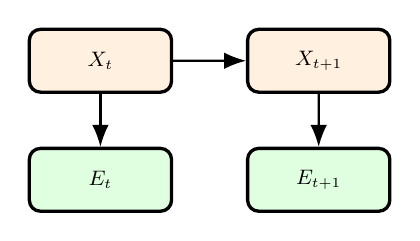
\begin{tikzpicture}[>=Latex, scale=0.84, every node/.style={font=\small, transform shape}]
      \node[hiddennode] (r1) at (0,1.0) {$X_t$};
      \node[evidnode] (u1) at (0,-0.8) {$E_t$};
      \node[hiddennode] (r2) at (3.3,1.0) {$X_{t+1}$};
      \node[evidnode] (u2) at (3.3,-0.8) {$E_{t+1}$};
      \draw[flowarrow] (r1) -- (r2);
      \draw[flowarrow] (r1) -- (u1);
      \draw[flowarrow] (r2) -- (u2);
    \end{tikzpicture}
    \end{center}
  \end{column}
\end{columns}
\end{frame}

\begin{frame}{What Pieces Does an HMM Need?}
\keyquestion{Which probability pieces define a full HMM?}
\begin{columns}[T,onlytextwidth]
  \begin{column}{0.31\textwidth}
    \small
    \begin{tcolorbox}[colback=plainbg,colframe=plainframe,boxrule=0.7pt,title=Initial model]
    $P(X_1)$\\
    where does the hidden state start?
    \end{tcolorbox}
  \end{column}
  \begin{column}{0.31\textwidth}
    \small
    \begin{tcolorbox}[colback=questionbg,colframe=questionframe,boxrule=0.7pt,title=Transition model]
    $P(X_t \mid X_{t-1})$\\
    how does state change?
    \end{tcolorbox}
  \end{column}
  \begin{column}{0.31\textwidth}
    \small
    \begin{tcolorbox}[colback=notationbg,colframe=notationframe,boxrule=0.7pt,title=Sensor model]
    $P(E_t \mid X_t)$\\
    how does evidence arise?
    \end{tcolorbox}
  \end{column}
\end{columns}
\plainidea{An HMM is fully specified by one initial model, one transition model, and one sensor model.}
\end{frame}

\begin{frame}{Small HMM Example: Rain and Umbrella}
\keyquestion{What do transition and sensor probabilities look like in a real small example?}
\small
\begin{columns}[T,onlytextwidth]
  \begin{column}{0.48\textwidth}
    \begin{center}
    \begin{tabular}{lcc}
    \toprule
    from / to & Rain & Dry \\
    \midrule
    Rain & 0.7 & 0.3 \\
    Dry  & 0.3 & 0.7 \\
    \bottomrule
    \end{tabular}
    \end{center}
    \begin{tcolorbox}[colback=plainbg,colframe=plainframe,boxrule=0.7pt,title=Transition idea]
    Weather tends to persist, but it can still change.
    \end{tcolorbox}
  \end{column}
  \begin{column}{0.48\textwidth}
    \begin{center}
    \begin{tabular}{lcc}
    \toprule
    state & $P(Umb{=}t)$ & $P(Umb{=}f)$ \\
    \midrule
    Rain & 0.9 & 0.1 \\
    Dry  & 0.2 & 0.8 \\
    \bottomrule
    \end{tabular}
    \end{center}
    \begin{tcolorbox}[colback=questionbg,colframe=questionframe,boxrule=0.7pt,title=Sensor idea]
    Umbrellas are strong clues for rain, but they are not perfect.
    \end{tcolorbox}
  \end{column}
\end{columns}
\plainidea{The model is probabilistic because state change and observation generation are both uncertain.}
\end{frame}

\begin{frame}{Kalman Filter}
\keyquestion{What if the hidden state is continuous instead of a small set of discrete labels?}
\begin{columns}[T,onlytextwidth]
  \begin{column}{0.54\textwidth}
    \begin{itemize}
      \item used for continuous quantities such as position, speed, or angle
      \item assumes linear dynamics and Gaussian noise
      \item repeatedly predicts and corrects, like filtering in an HMM
    \end{itemize}
    \begin{tcolorbox}[colback=plainbg,colframe=plainframe,boxrule=0.7pt,title=Example]
    robot position tracking, GPS fusion, sensor smoothing
    \end{tcolorbox}
  \end{column}
  \begin{column}{0.42\textwidth}
    \begin{center}
    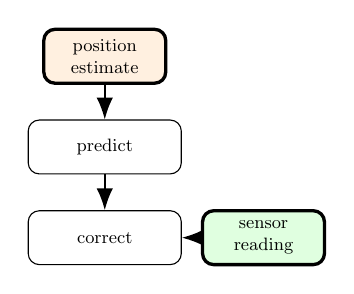
\begin{tikzpicture}[>=Latex, scale=0.72, every node/.style={font=\small, transform shape}]
      \node[hiddennode] (x1) at (0,1.5) {position\\estimate};
      \node[softbox] (p) at (0,-0.1) {predict};
      \node[softbox] (c) at (0,-1.7) {correct};
      \node[evidnode] (z) at (2.8,-1.7) {sensor\\reading};
      \draw[flowarrow] (x1) -- (p);
      \draw[flowarrow] (p) -- (c);
      \draw[flowarrow] (z) -- (c);
    \end{tikzpicture}
    \end{center}
  \end{column}
\end{columns}
\plainidea{Kalman filtering is the continuous-state relative of HMM-style filtering.}
\end{frame}

\begin{frame}{HMM or Kalman Filter?}
\keyquestion{How do we know which temporal model is more suitable?}
\small
\begin{center}
\scriptsize
\begin{tabular}{>{\raggedright\arraybackslash}p{0.20\textwidth} >{\raggedright\arraybackslash}p{0.28\textwidth} >{\raggedright\arraybackslash}p{0.28\textwidth}}
\toprule
feature & HMM & Kalman filter \\
\midrule
hidden state & discrete labels & continuous values \\
example & rain / dry & position / velocity \\
observations & categorized evidence & numeric readings \\
assumption & discrete transitions & linear Gaussian dynamics \\
\bottomrule
\end{tabular}
\end{center}
\plainidea{Use HMMs for discrete states and Kalman filters for continuous states.}
\end{frame}

\begin{frame}{What Is a Dynamic Bayesian Network?}
\keyquestion{What if one time step contains several hidden and observed variables?}
\begin{columns}[T,onlytextwidth]
  \begin{column}{0.52\textwidth}
    \begin{itemize}
      \item a dynamic Bayesian network (DBN) generalises the HMM
      \item each time step can contain several variables
      \item arrows can exist within a time step and across time steps
    \end{itemize}
  \end{column}
  \begin{column}{0.44\textwidth}
    \begin{center}
    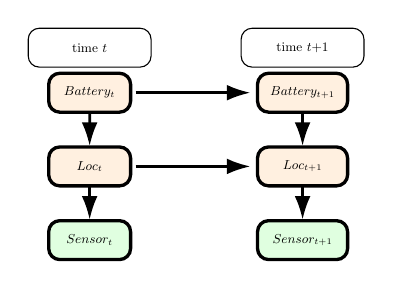
\begin{tikzpicture}[>=Latex, scale=0.52, every node/.style={font=\small, transform shape}]
      \node[note] at (0,2.9) {time $t$};
      \node[note] at (5.2,2.9) {time $t{+}1$};
      \node[hiddennode, minimum width=2.0cm] (b1) at (0,1.8) {$Battery_t$};
      \node[hiddennode, minimum width=2.0cm] (l1) at (0,0.0) {$Loc_t$};
      \node[evidnode, minimum width=2.0cm] (s1) at (0,-1.8) {$Sensor_t$};
      \node[hiddennode, minimum width=2.2cm] (b2) at (5.2,1.8) {$Battery_{t+1}$};
      \node[hiddennode, minimum width=2.2cm] (l2) at (5.2,0.0) {$Loc_{t+1}$};
      \node[evidnode, minimum width=2.2cm] (s2) at (5.2,-1.8) {$Sensor_{t+1}$};
      \draw[-{Latex[length=3mm,width=2mm]}, line width=1pt] (b1) -- (l1);
      \draw[-{Latex[length=3mm,width=2mm]}, line width=1pt] (l1) -- (s1);
      \draw[-{Latex[length=3mm,width=2mm]}, line width=1pt] (b2) -- (l2);
      \draw[-{Latex[length=3mm,width=2mm]}, line width=1pt] (l2) -- (s2);
      \draw[-{Latex[length=3mm,width=2mm]}, line width=1pt] ($(b1.east)+(0.10,0)$) -- ($(b2.west)+(-0.15,0)$);
      \draw[-{Latex[length=3mm,width=2mm]}, line width=1pt] ($(l1.east)+(0.10,0)$) -- ($(l2.west)+(-0.15,0)$);
    \end{tikzpicture}
    \end{center}
  \end{column}
\end{columns}
\plainidea{A dynamic Bayesian network (DBN) repeats a small Bayesian network across time.}
\end{frame}

\begin{frame}{DBN Example: Robot Tracking}
\keyquestion{Why is a DBN more suitable than a simple HMM for many real systems?}
\begin{columns}[T,onlytextwidth]
  \begin{column}{0.50\textwidth}
    \small
    \begin{tcolorbox}[colback=plainbg,colframe=plainframe,boxrule=0.7pt,title=Hidden variables]
    location, velocity, battery level
    \end{tcolorbox}
    \begin{tcolorbox}[colback=questionbg,colframe=questionframe,boxrule=0.7pt,title=Observed variables]
    GPS, odometry, battery meter
    \end{tcolorbox}
    \begin{tcolorbox}[colback=notationbg,colframe=notationframe,boxrule=0.7pt,title=Why useful?]
    Different hidden variables influence one another inside the same time step.
    \end{tcolorbox}
  \end{column}
  \begin{column}{0.46\textwidth}
    \begin{center}
    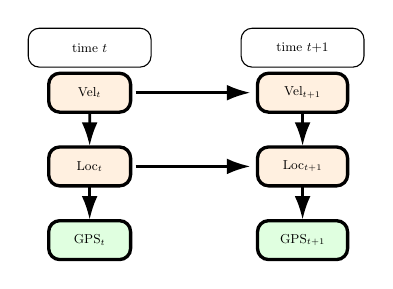
\begin{tikzpicture}[>=Latex, scale=0.52, every node/.style={font=\small, transform shape}]
      \node[note] at (0,2.9) {time $t$};
      \node[note] at (5.2,2.9) {time $t{+}1$};
      \node[hiddennode, minimum width=2.0cm] (v1) at (0,1.8) {Vel$_t$};
      \node[hiddennode, minimum width=2.0cm] (x1) at (0,0.0) {Loc$_t$};
      \node[evidnode, minimum width=2.0cm] (g1) at (0,-1.8) {GPS$_t$};
      \node[hiddennode, minimum width=2.2cm] (v2) at (5.2,1.8) {Vel$_{t+1}$};
      \node[hiddennode, minimum width=2.2cm] (x2) at (5.2,0.0) {Loc$_{t+1}$};
      \node[evidnode, minimum width=2.2cm] (g2) at (5.2,-1.8) {GPS$_{t+1}$};
      \draw[-{Latex[length=3mm,width=2mm]}, line width=1pt] (v1) -- (x1);
      \draw[-{Latex[length=3mm,width=2mm]}, line width=1pt] (x1) -- (g1);
      \draw[-{Latex[length=3mm,width=2mm]}, line width=1pt] (v2) -- (x2);
      \draw[-{Latex[length=3mm,width=2mm]}, line width=1pt] (x2) -- (g2);
      \draw[-{Latex[length=3mm,width=2mm]}, line width=1pt] ($(v1.east)+(0.10,0)$) -- ($(v2.west)+(-0.15,0)$);
      \draw[-{Latex[length=3mm,width=2mm]}, line width=1pt] ($(x1.east)+(0.10,0)$) -- ($(x2.west)+(-0.15,0)$);
    \end{tikzpicture}
    \end{center}
  \end{column}
\end{columns}
\plainidea{A DBN lets us represent several related hidden and observed variables at once.}
\end{frame}

\begin{frame}{Exact or Approximate Inference Over Time?}
\keyquestion{Do temporal models always allow exact inference?}
\begin{columns}[T,onlytextwidth]
  \begin{column}{0.48\textwidth}
    \begin{tcolorbox}[colback=plainbg,colframe=plainframe,boxrule=0.7pt,title=Exact inference]
    forward algorithm\\
    forward-backward\\
    Viterbi
    \end{tcolorbox}
  \end{column}
  \begin{column}{0.48\textwidth}
    \begin{tcolorbox}[colback=questionbg,colframe=questionframe,boxrule=0.7pt,title=Approximate inference]
    likelihood weighting\\
    particle filtering\\
    other sampling methods
    \end{tcolorbox}
  \end{column}
\end{columns}
\plainidea{Small models can often use exact inference. Larger or more complex temporal models often need approximate inference.}
\end{frame}

\begin{frame}{Why Does Approximate Inference Become Useful?}
\keyquestion{What makes exact temporal inference expensive?}
\begin{center}
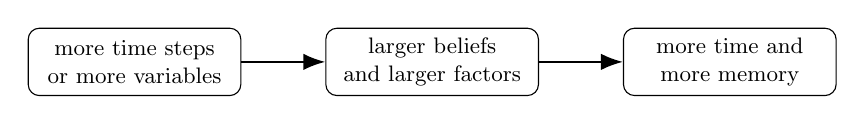
\begin{tikzpicture}[>=Latex, scale=0.9, every node/.style={font=\small, transform shape}]
  \node[softbox, minimum width=3.0cm] (s1) at (0,0) {more time steps\\or more variables};
  \node[softbox, minimum width=3.0cm] (s2) at (4.2,0) {larger beliefs\\and larger factors};
  \node[softbox, minimum width=3.0cm] (s3) at (8.4,0) {more time and\\more memory};
  \draw[flowarrow] (s1) -- (s2);
  \draw[flowarrow] (s2) -- (s3);
\end{tikzpicture}
\end{center}
\begin{tcolorbox}[colback=questionbg,colframe=questionframe,boxrule=0.7pt]
Particle filtering is common when the state space is large, continuous, or hard to sum over exactly.
\end{tcolorbox}
\plainidea{Approximate methods are not second-best by design. They are often the only practical choice in realistic temporal systems.}
\end{frame}

\begin{frame}{Temporal Reasoning in Intelligent Systems}
\keyquestion{Where do we actually use these models outside textbook weather examples?}
\begin{columns}[T,onlytextwidth]
  \begin{column}{0.48\textwidth}
    \begin{tcolorbox}[colback=plainbg,colframe=plainframe,boxrule=0.7pt,title=Robotics,fontupper=\small]
    track pose, velocity, and obstacles from noisy sensors
    \end{tcolorbox}
    \begin{tcolorbox}[colback=questionbg,colframe=questionframe,boxrule=0.7pt,title=Transport,fontupper=\small]
    track congestion and predict delays from live feeds
    \end{tcolorbox}
  \end{column}
  \begin{column}{0.48\textwidth}
    \begin{tcolorbox}[colback=notationbg,colframe=notationframe,boxrule=0.7pt,title=Energy systems,fontupper=\small]
    track load, faults, and risk from streaming sensors
    \end{tcolorbox}
    \begin{tcolorbox}[colback=plainbg,colframe=plainframe,boxrule=0.7pt,title=Healthcare monitoring,fontupper=\small]
    track patient condition from noisy measurements
    \end{tcolorbox}
  \end{column}
\end{columns}
\plainidea{These models help when true state changes over time and evidence is noisy.}
\end{frame}

\begin{frame}{Applied Example: Robot Localization}
\keyquestion{What do filtering and prediction look like in a robot system?}
\begin{columns}[T,onlytextwidth]
  \begin{column}{0.54\textwidth}
    \begin{tcolorbox}[colback=plainbg,colframe=plainframe,boxrule=0.7pt,title=System view,fontupper=\small]
    Hidden state: robot pose and velocity\\
    Evidence: GPS, camera, lidar, odometry
    \end{tcolorbox}
    \begin{tcolorbox}[colback=notationbg,colframe=notationframe,boxrule=0.7pt,title=Role,fontupper=\small]
    filtering stabilizes belief; prediction supports planning
    \end{tcolorbox}
  \end{column}
  \begin{column}{0.42\textwidth}
    \begin{center}
    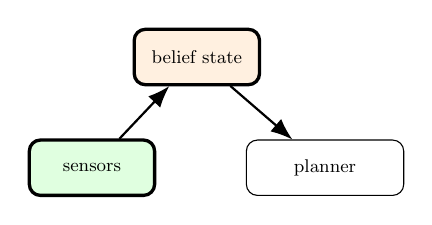
\begin{tikzpicture}[>=Latex, scale=0.74, every node/.style={font=\small, transform shape}]
      \node[hiddennode] (b) at (0,1.0) {belief state};
      \node[evidnode] (s1) at (-1.8,-0.9) {sensors};
      \node[softbox] (p) at (2.2,-0.9) {planner};
      \draw[flowarrow] (s1) -- (b);
      \draw[flowarrow] (b) -- (p);
    \end{tikzpicture}
    \end{center}
  \end{column}
\end{columns}
\plainidea{The planner should act on filtered belief, not on one noisy reading.}
\end{frame}

\begin{frame}{Applied Example: Smart Transport Forecasting}
\keyquestion{What is the hidden state in a live transport monitoring system?}
\begin{columns}[T,onlytextwidth]
  \begin{column}{0.54\textwidth}
    \begin{tcolorbox}[colback=plainbg,colframe=plainframe,boxrule=0.7pt,title=System view,fontupper=\small]
    Hidden state: demand, disruption severity, congestion level\\
    Evidence: GPS traces, ticketing, incident reports
    \end{tcolorbox}
    \begin{tcolorbox}[colback=notationbg,colframe=notationframe,boxrule=0.7pt,title=Role,fontupper=\small]
    prediction estimates delay risk before visible failure
    \end{tcolorbox}
  \end{column}
  \begin{column}{0.42\textwidth}
    \begin{center}
    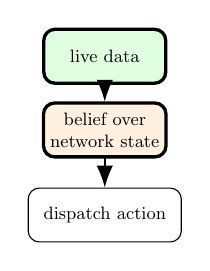
\begin{tikzpicture}[>=Latex, scale=0.72, every node/.style={font=\small, transform shape}]
      \node[evidnode] (e) at (0,1.1) {live data};
      \node[hiddennode] (h) at (0,-0.2) {belief over\\network state};
      \node[softbox] (a) at (0,-1.7) {dispatch action};
      \draw[flowarrow] (e) -- (h);
      \draw[flowarrow] (h) -- (a);
    \end{tikzpicture}
    \end{center}
  \end{column}
\end{columns}
\plainidea{Prediction helps the system respond before disruption becomes obvious.}
\end{frame}

\begin{frame}{Failure Modes in Temporal Reasoning}
\keyquestion{What can go wrong if the temporal model or the evidence stream is poor?}
\begin{columns}[T,onlytextwidth]
  \begin{column}{0.48\textwidth}
    \begin{tcolorbox}[colback=questionbg,colframe=questionframe,boxrule=0.7pt,title=Common problems]
    sensor drift\\
    missing data\\
    abrupt regime change\\
    overconfident beliefs
    \end{tcolorbox}
  \end{column}
  \begin{column}{0.48\textwidth}
    \begin{tcolorbox}[colback=plainbg,colframe=plainframe,boxrule=0.7pt,title=Why it matters]
    a bad temporal belief can lead to bad planning, late alerts, or unsafe action selection
    \end{tcolorbox}
  \end{column}
\end{columns}
\plainidea{The belief state is only as good as the model assumptions and the evidence stream behind it.}
\end{frame}

\begin{frame}{Simple Mitigation Ideas}
\keyquestion{How do we reduce temporal reasoning errors in practice?}
\begin{columns}[T,onlytextwidth]
  \begin{column}{0.48\textwidth}
    \begin{tcolorbox}[colback=plainbg,colframe=plainframe,boxrule=0.7pt,title=Model-side actions]
    recalibration\\
    drift monitoring\\
    fallback models
    \end{tcolorbox}
  \end{column}
  \begin{column}{0.48\textwidth}
    \begin{tcolorbox}[colback=questionbg,colframe=questionframe,boxrule=0.7pt,title=Decision-side actions]
    be more conservative when uncertainty is high\\
    wait for more evidence before irreversible actions
    \end{tcolorbox}
  \end{column}
\end{columns}
\plainidea{Good systems track uncertainty, not just the most likely state estimate.}
\end{frame}

\begin{frame}{Where Are We Going Next?}
\keyquestion{What changes when we move from tracking belief to choosing actions?}
\begin{columns}[T,onlytextwidth]
  \begin{column}{0.52\textwidth}
    \begin{tcolorbox}[colback=plainbg,colframe=plainframe,boxrule=0.7pt,title=Today,fontupper=\small]
    hidden-state tracking over time\\
    infer what is happening now
    \end{tcolorbox}
    \begin{tcolorbox}[colback=questionbg,colframe=questionframe,boxrule=0.7pt,title=Next lecture,fontupper=\small]
    combine belief, utility, and action\\
    decide what to do
    \end{tcolorbox}
  \end{column}
  \begin{column}{0.42\textwidth}
    \begin{center}
    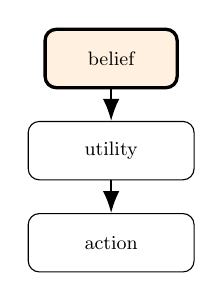
\begin{tikzpicture}[>=Latex, scale=0.78, every node/.style={font=\small, transform shape}]
      \node[hiddennode] (b) at (0,0.9) {belief};
      \node[softbox] (u) at (0,-0.6) {utility};
      \node[softbox] (a) at (0,-2.1) {action};
      \draw[flowarrow] (b) -- (u);
      \draw[flowarrow] (u) -- (a);
    \end{tikzpicture}
    \end{center}
  \end{column}
\end{columns}
\plainidea{Day 4 moves from belief tracking to action choice under uncertainty.}
\end{frame}

\begin{frame}{Key Takeaways}
\begin{itemize}
  \item temporal models track hidden state as new evidence arrives
  \item filtering, prediction, smoothing, and Viterbi answer different time-based questions
  \item HMMs are the basic discrete temporal model
  \item Kalman filters support continuous hidden states
  \item DBNs generalize temporal reasoning to several related variables per time step
\end{itemize}
\plainidea{Students should now see temporal probabilistic reasoning as a belief-update process over time, not just a list of new algorithms.}
\end{frame}

\begin{frame}{In-Class Exercises}
\exercisebreakcontent{Use the exercise time to say clearly which temporal query or model fits each scenario and why.}
\end{frame}

\begin{frame}{Further Study}
\begin{itemize}
  \item Read Poole Chapter 9 and AIMA Chapter 14.
  \item Practice: Poole Ch.9, Exercises 9.13, 9.14, and 9.17.
  \item AIMA probabilistic-reasoning-over-time exercise page: 15.1, 15.2, 15.3, 15.13, and 15.20.
  \item Focus on filtering, smoothing, Viterbi-style sequence reasoning, and when continuous-state models are needed.
\end{itemize}
\end{frame}

\end{document}
